\documentclass[12pt]{article}
\usepackage[english]{babel}
\usepackage{natbib}
\usepackage{lipsum}
\usepackage{fontawesome}
\usepackage{hyperref}
\usepackage{circuitikz}
\usepackage{url}
\usepackage{placeins}
\usepackage[utf8x]{inputenc} 
\usepackage{amsmath}
\usepackage{graphicx}

\graphicspath{{images/}}
\usepackage{parskip}
\usepackage{fancyhdr}
\usepackage{vmargin}
\usepackage{wrapfig}
\usepackage{subfig}

\usepackage{siunitx}


\setmarginsrb{3 cm}{2.5 cm}{3 cm}{2.5 cm}{1 cm}{1.5 cm}{1 cm}{1.5 cm}


%%%%%%%% to embed code %%%%%%%%%%%%%%
\usepackage{listings}
\usepackage{color}
\definecolor{dkgreen}{rgb}{0,0.6,0}
\definecolor{gray}{rgb}{0.5,0.5,0.5}
\definecolor{mauve}{rgb}{0.58,0,0.82}
\lstset{
  language=Java,
  aboveskip=3mm,
  belowskip=3mm,
  showstringspaces=false,
  columns=flexible,
  basicstyle={\small\ttfamily},
  numberstyle=\tiny\color{gray},
  keywordstyle=\color{blue},
  commentstyle=\color{dkgreen},
  stringstyle=\color{mauve},
  breaklines=true,
  breakatwhitespace=true,
  tabsize=3,
  numbers=left,
  xleftmargin=2em,
  frame=single,
  framexleftmargin=1.5em
}

%%%%%%%% to embed code %%%%%%%%%%%%%%


\title{Portable Heart Rate Monitor}	% Title  
\author{EN1093 - Laboratory Practice}	%Author
\date{\today}						% Date

\makeatletter
\let\thetitle\@title
\let\theauthor\@author
\let\thedate\@date
\makeatother

\pagestyle{fancy}
\fancyhf{}
\rhead{\theauthor}
\lhead{\thetitle}
\cfoot{\thepage}

\begin{document}

%%%%%%%%%%%%%%%%%%%%%%%%%%%%%%%%%%%%%%%%%%%%%%%%%%%%%%%%%%%%%%%%%%%%%%%%%%%%%%%%%%%%%%%%

\begin{titlepage}
	
	\centering
	
	\textsc{\small DEPARTMENT OF ELECTRONIC AND TELECOMMUNICATION ENGINEERING\\}
	\textsc{\small UNIVERSITY OF MORATUWA}\\[1.0 cm]
    \vspace*{0.5 cm}
    
\includegraphics[scale = 0.35]{uom.png}\\[1.5 cm]	% University Logo
    \textsc{\LARGE Group Project Report}\\[0.7 cm]	% University Name 
	\textsc{\Large EN1093 - Laboratory Practice}\\[0.5 cm]			% Course Code

	\rule{\linewidth}{0.2 mm} \\[0.4 cm]
	{ \huge \bfseries \thetitle}\\
	\rule{\linewidth}{0.2 mm} \\[1.5 cm]
	
	\begin{minipage}{0.4\textwidth}
		\begin{flushleft} \large
			\emph{Authors:}\\
			K.K. Herath\\
			H.M.U.D Herath\\
			R.U. Hettiarachchi\\
			M.N. Hettiaratchchi
			\end{flushleft}
			\end{minipage}~
			\begin{minipage}{0.4\textwidth}
			\begin{flushright} \large
			\emph{Registration Number:} \\
			170213V\\
			170215U\\
			170221T\\
			170222X
		\end{flushright}
	\end{minipage}\\[2 cm]
	 This is submitted as a partial fulfillment for the module EN1093\\[0.2 cm]
	 ---\\
	{\large \thedate}\\[2 cm]
	
	\vfill
	
\end{titlepage}

\newpage
\section{Abstract}
The proposed project measures the heart rate of a person using optical sensors. 
The optical sensor detects the variation of blood volume at the fingertip.
In our project the sensor will be an infrared light emitting diode (IR LED) which will be on the same side of the finger.
The underlying principle is that the intensity of the reflected infrared light varies on the blood volume at an instance of the fingertip, which changes proportionately to each cardiac cycle. 
The lighting condition in the environment is very important to avoid distortion in the signal so we have taken the following measures,

• To design a special enclosure to cover the optical sensor for accurate measurements

• To use a band filter to remove unnecessary wavelengths.

Based on the refined output signal, we used an Atmel microcontroller to calculate and display the heart rate through the LCD Display.

\section{Acknowledgement}
We would like to express our gratitude to our supervisor Mr.Asanka Rathnayake for giving us technical advice and guidance.\\
Our sincere thanks goes to Mr.Thilina Sameera Ambagahawaththa for the inspiration and advice given to us to compile this report in LaTeX.

We pay our gratitude to all the lecturers, instructors and other academic staff who intimately welcomed us to share their knowledge and experiences. We are very grateful to the personnel who are in charge of laboratories for allowing us to use the laboratories when needed and for the support given to solve technical problems.

%%%%%%%%%%%%%%%%%%%%%%%%%%%%%%%%%%%%%%%%%%%%%%%%%%%%%%%%%%%%%%%%%%%%%%%%%%%%%%%%%%%%%%%%%
\newpage
\tableofcontents
\pagebreak
%%%%%%%%%%%%%%%%%%%%%%%%%%%%%%%%%%%%%%%%%%%%%%%%%%%%%%%%%%%%%%%%%%%%%%%%%%%%%%%%%%%%%%%%%


%%%%%%%%%%%%%%%%%%%%%%%%%%%%%%%%%%%%%%%%%%%%%%%%%%%%%%%%%%%%%%%%%%%%%%%%%%%%%%%%%%%%%%%%%
\section{Introduction}
This is a simple report template with the UCT logo. Feel free to use/modify it to suit your needs. Variables that need to be altered have been commented to make modifications easier. For example if you need to change the university logo, look for the comment \texttt{\% University Logo} in this file and then make appropriate modifications in that line.
A Table of Contents and a bibliography have also been implemented. To add entries to your bibliography, simply edit \texttt{biblist.bib} in the root folder and then use the \texttt{\textbackslash cite\{\ldots\}} command in \texttt{main.tex} \cite{ppg_wiki}. The Table of Contents will be updated automatically.
I hope that you find this template both visually appealing and useful. \\
\hspace{1 cm}--- Linus

%%%%%%%%%%%%%%%%%%%%%%%%%%%%%%%%%%%%%%%%%%%%%%%%%%%%%%%%%%%%%%%%%%%%%%%%%%%%%%%%%%%%%%%%%








%%%%%%%%%%%%%%%%%%%%%%%%%%%%%%%%%%%%%%%%%%%%%%%%%%%%%%%%%%%%%%%%%%
\newpage
\section{Methodology}

	The methodology can be summarized to the following block diagram.


	\subsection{Sensor}
	\lipsum[5]
	\begin{figure}[!htbp]  %this figure will be at the right

		\centering
		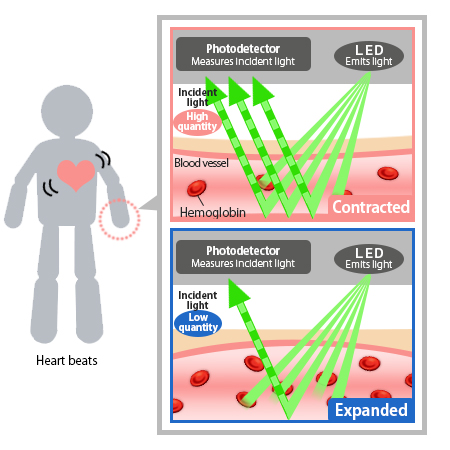
\includegraphics[width=0.65\textwidth]{sensing.jpg}
		\caption{How IR LED light is reflected from the blood vessels}
	\end{figure}


		\subsection{Amplification and Filtering}
		
		To amplify the PPG signal we designed an amplifier circuit. However we observed that without proper filtering we cannot get a clear signal due to noise.
		So we had to determine the necessary values for the filter circuit.\\
		The typical heart rate of an adult is between 60-100bpm\cite{typical_pulse}.In frequency terms, these values correspond to the range 1-1.7 Hz.So an active bandpass filter circuit was designed to provide the following characteristics using LM358.


\subsubsection{Calculations}
\label{sec:4.2.1}
\begin{center}
	Cutoff frequency ($f$) = $\frac{1}{2\pi RC}$
	
	
	
	Lower cutoff frequency =$\ \frac{1}{2\pi ( 680\ k\si{\ohm}\ )( 100\ nF)}$ = 2.34051 Hz
	
	
	
	Upper cutoff frequency =$\ \frac{1}{2 \pi  ( 47\ k\si{\ohm})( 4.7\ \si{\micro}F)}$ = 0.720484 Hz
	\end{center}
	
	
	
	
	
	So we have,

		\begin{itemize}
			\item Gain of 10
			\item Lower Cutoff Frequency of 0.72 Hz
			\item Upper Cutoff Frequency of 2.34 Hz\\
		  \end{itemize}
		 To have a low powered operational amplifier we selected LM358 integrated circuit.
	
		\begin{figure}[!htbp]
			\includegraphics[width=\textwidth]{LM358-Bandpass}
			\caption{Active bandpass filter for the pulse sensor}
		\end{figure}
	
		\clearpage
	\subsection{Calculating BPM from the analog signal}
	The ATMega32 microcontroller was used to sample the analog signal to 0-1023 voltage levels. Then an algorithm was developed to identify peaks and thereby calculate the beats per minute. We used Atmel Studio to compile and flash the hex file to the microcontroller. 


	\subsubsection{Microcontroller}
	The ATmega32 is a low power high performance atmel AVR 8-bit microcontroller.
			\begin{figure}[!htbp]
				\centering
				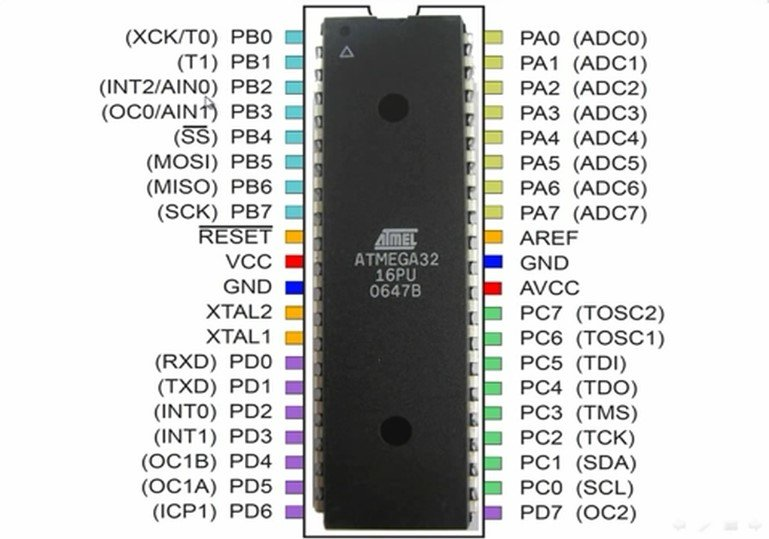
\includegraphics[scale = 1]{atmega32.jpg}
				\caption{ATmega32 pinout}
			\end{figure}

	\subsubsection{Obtaining a threshold value}
	\label{sec:4.3.2}

	Give basic info on how threshold was determined.

	\subsubsection{Algorithm}
	can include the flowchat, and code here

	\begin{lstlisting}
		/*  Group 7 | UoM | ENTC 17Batch  */
		#ifndef F_CPU
		#define F_CPU 16000000UL // 16 MHz clock speed
		#endif
		#define D0 eS_PORTD0
		#define D1 eS_PORTD1
		#define D2 eS_PORTD2
		#define D3 eS_PORTD3
		#define D4 eS_PORTD4
		#define D5 eS_PORTD5
		#define D6 eS_PORTD6
		#define D7 eS_PORTD7
		#define RS eS_PORTC6
		#define EN eS_PORTC7
		
		#include <avr/io.h>
		#include <util/delay.h>
		#include "stdlib.h"
		#include "string.h"
		#include "lcd.h"
		
		char disp[16]="0000000000000001";
		char result[8] = "00000001"; 
		
		void lcd_disp(char arr[],int r,int c,char w[]){
			if(w=="clear")Lcd8_Clear();
			Lcd8_Set_Cursor(r,c);
			Lcd8_Write_String(arr);
		}
		
		void ADC_Init(){
			DDRA=0x0;			/* Make ADC port as input */
			ADCSRA = 0x87;			/* Enable ADC, fr/128  */
			ADMUX = 0x40;			/* Vref: Avcc, ADC channel: 0 */
		}
		
		int ADC_Read(char channel){
			int Ain,AinLow;
			
			ADMUX=ADMUX|(channel & 0x0f);	/* Set input channel to read */
		
			ADCSRA |= (1<<ADSC);		/* Start conversion */
			while((ADCSRA&(1<<ADIF))==0);	/* Monitor end of conversion interrupt */
			_delay_us(10);
			AinLow = (int)ADCL;		/* Read lower byte*/
			Ain = (int)ADCH*256;		/* Read higher 2 bits and 
							Multiply with weight */
			Ain = Ain + AinLow;				
			return(Ain);			/* Return digital value*/
		}
		
		 
		
		int main(void){
		
			DDRD = 0xFF;  // #
			DDRC = 0xFF;  //for lcd
			DDRA = 0x00;  //Analog input
			
			ADC_Init();
			
			Lcd8_Init(); //Initializing the LCD screen
			lcd_disp("Starting Pulse ~)",1,0,"");
			lcd_disp("Meter",2,0,"");
			
			_delay_ms(3000);
			int i;
		
			for(i=0;i>=0;i++){	
				
				char temp[11]="Analog - ";
				char val[4]; // 0 - 255 value
	
				itoa(ADC_Read(0),val,10);
		
				strcat(temp,val);
		
				lcd_disp(temp,1,0,"clear");
				_delay_ms(300);
			
			}	
		}
		
		\end{lstlisting}
		Based on this \cite{avr_analog} and this data-sheet \cite{atmega32_datasheet}
		%% Calibration and Ambient Lighting conditions %% 


\subsection{Enclosure and PCB Design}

	




\newpage
\section{Implementation and Results}


\subsection{The effect of noise on the signal}
Initially our goal was to amplify the signal received from the photodiodes. Then we observed that we could not receive a clear amplified heartbeat signal as it gets suppressed by the 50Hz noise signal.

\subsubsection{Without the filter - Dominant 50Hz noise}

\begin{figure}[!htbp]
	\begin{tabular}{cc}
	\centering

	\subfloat[oscilloscope output]{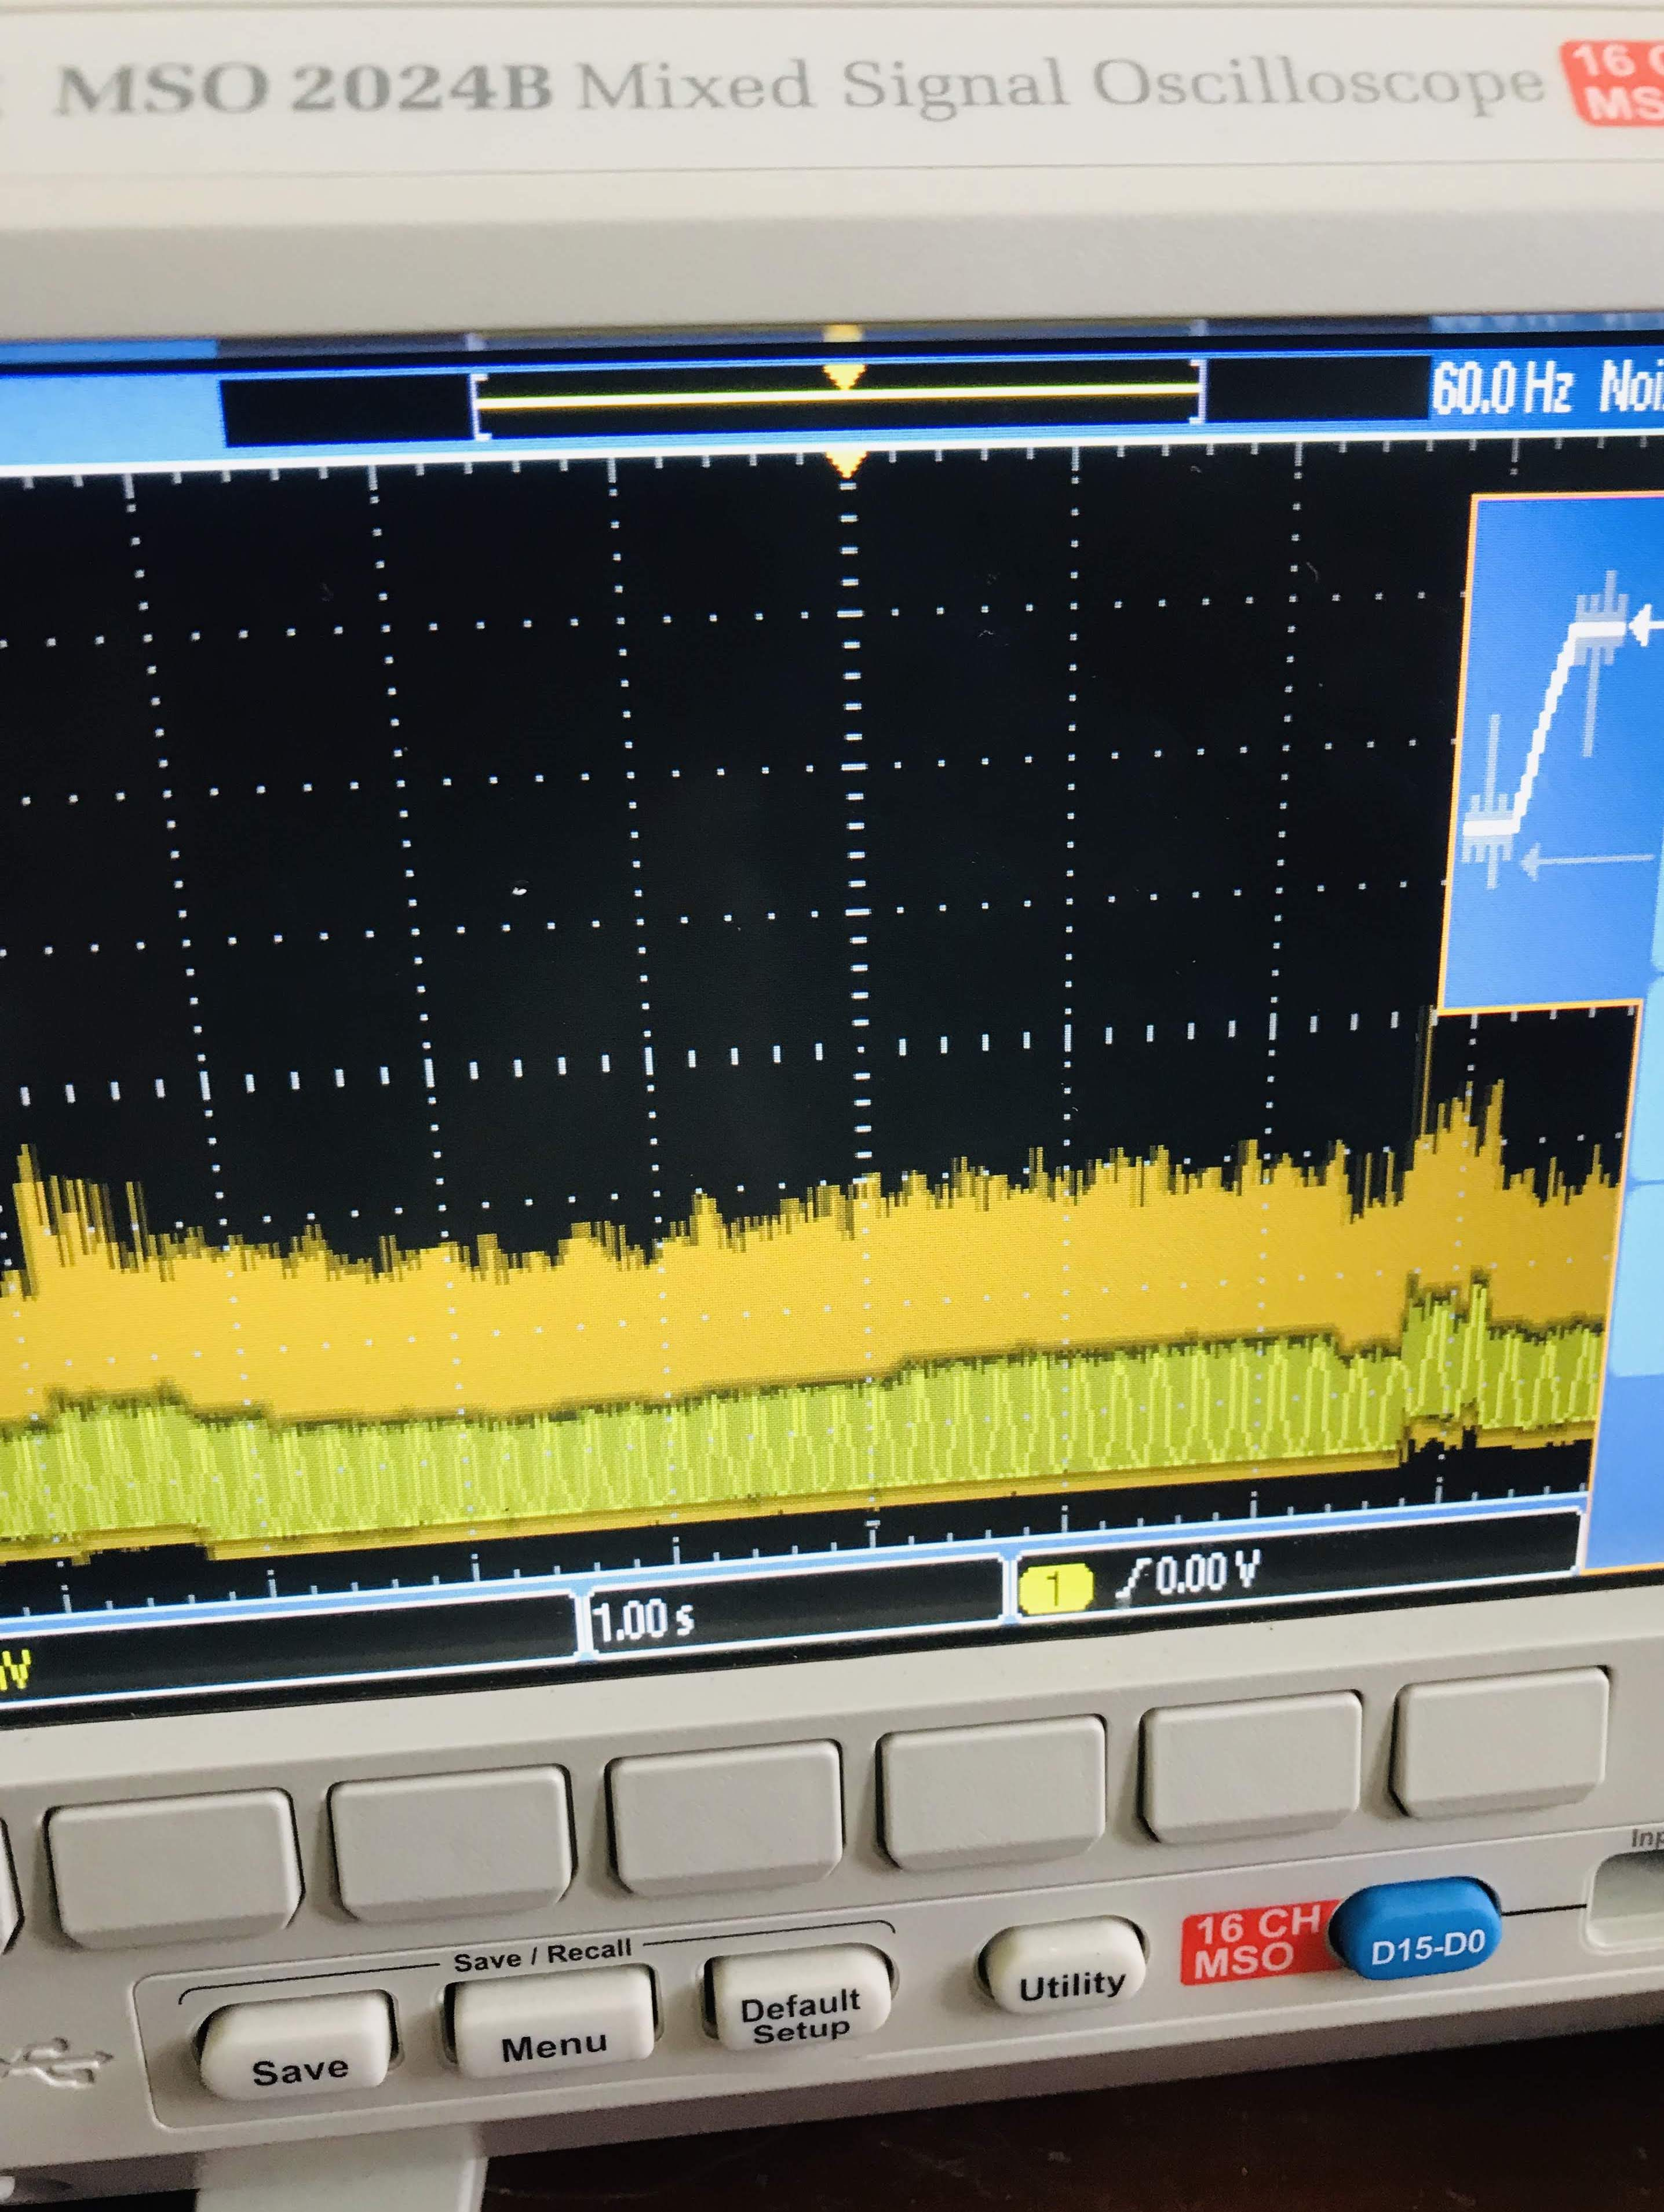
\includegraphics[width = 3in]{50Hz.jpg}}&
\subfloat[zoomed view]{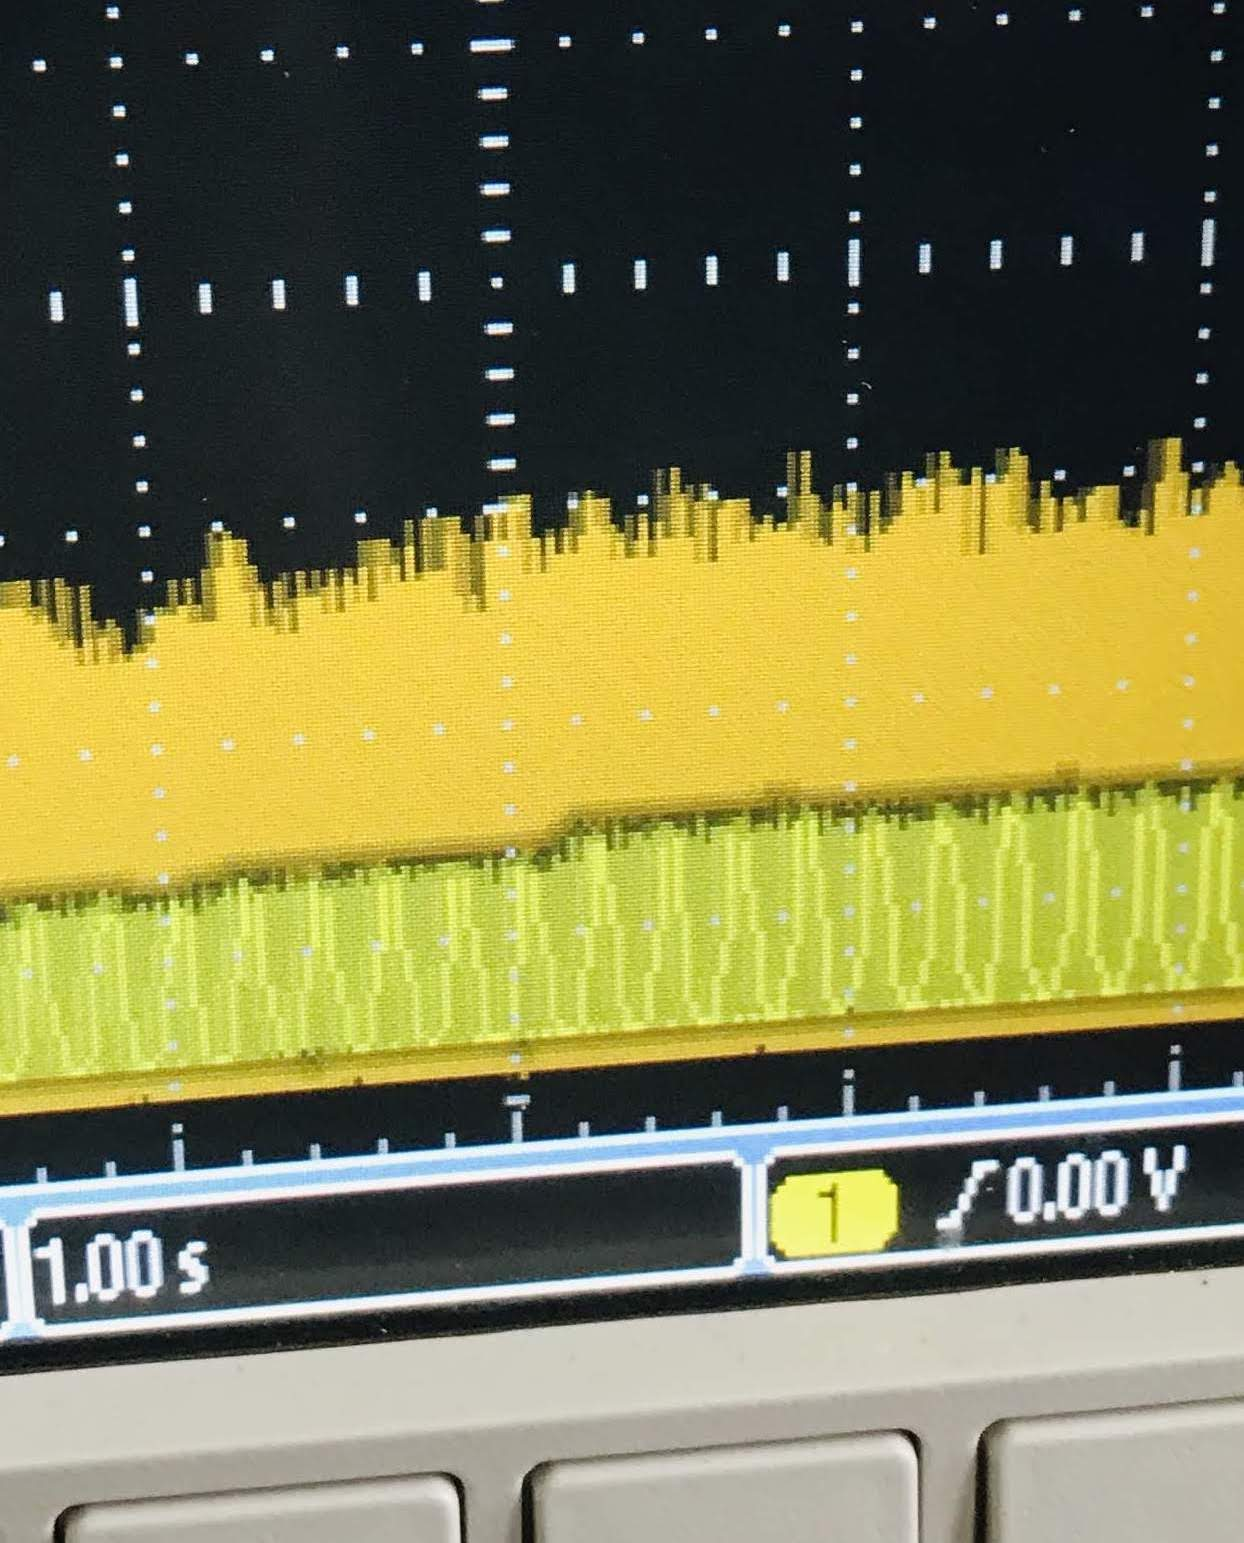
\includegraphics[width = 3in]{50Hz-z.jpg}}\\


	\end{tabular}
\end{figure}

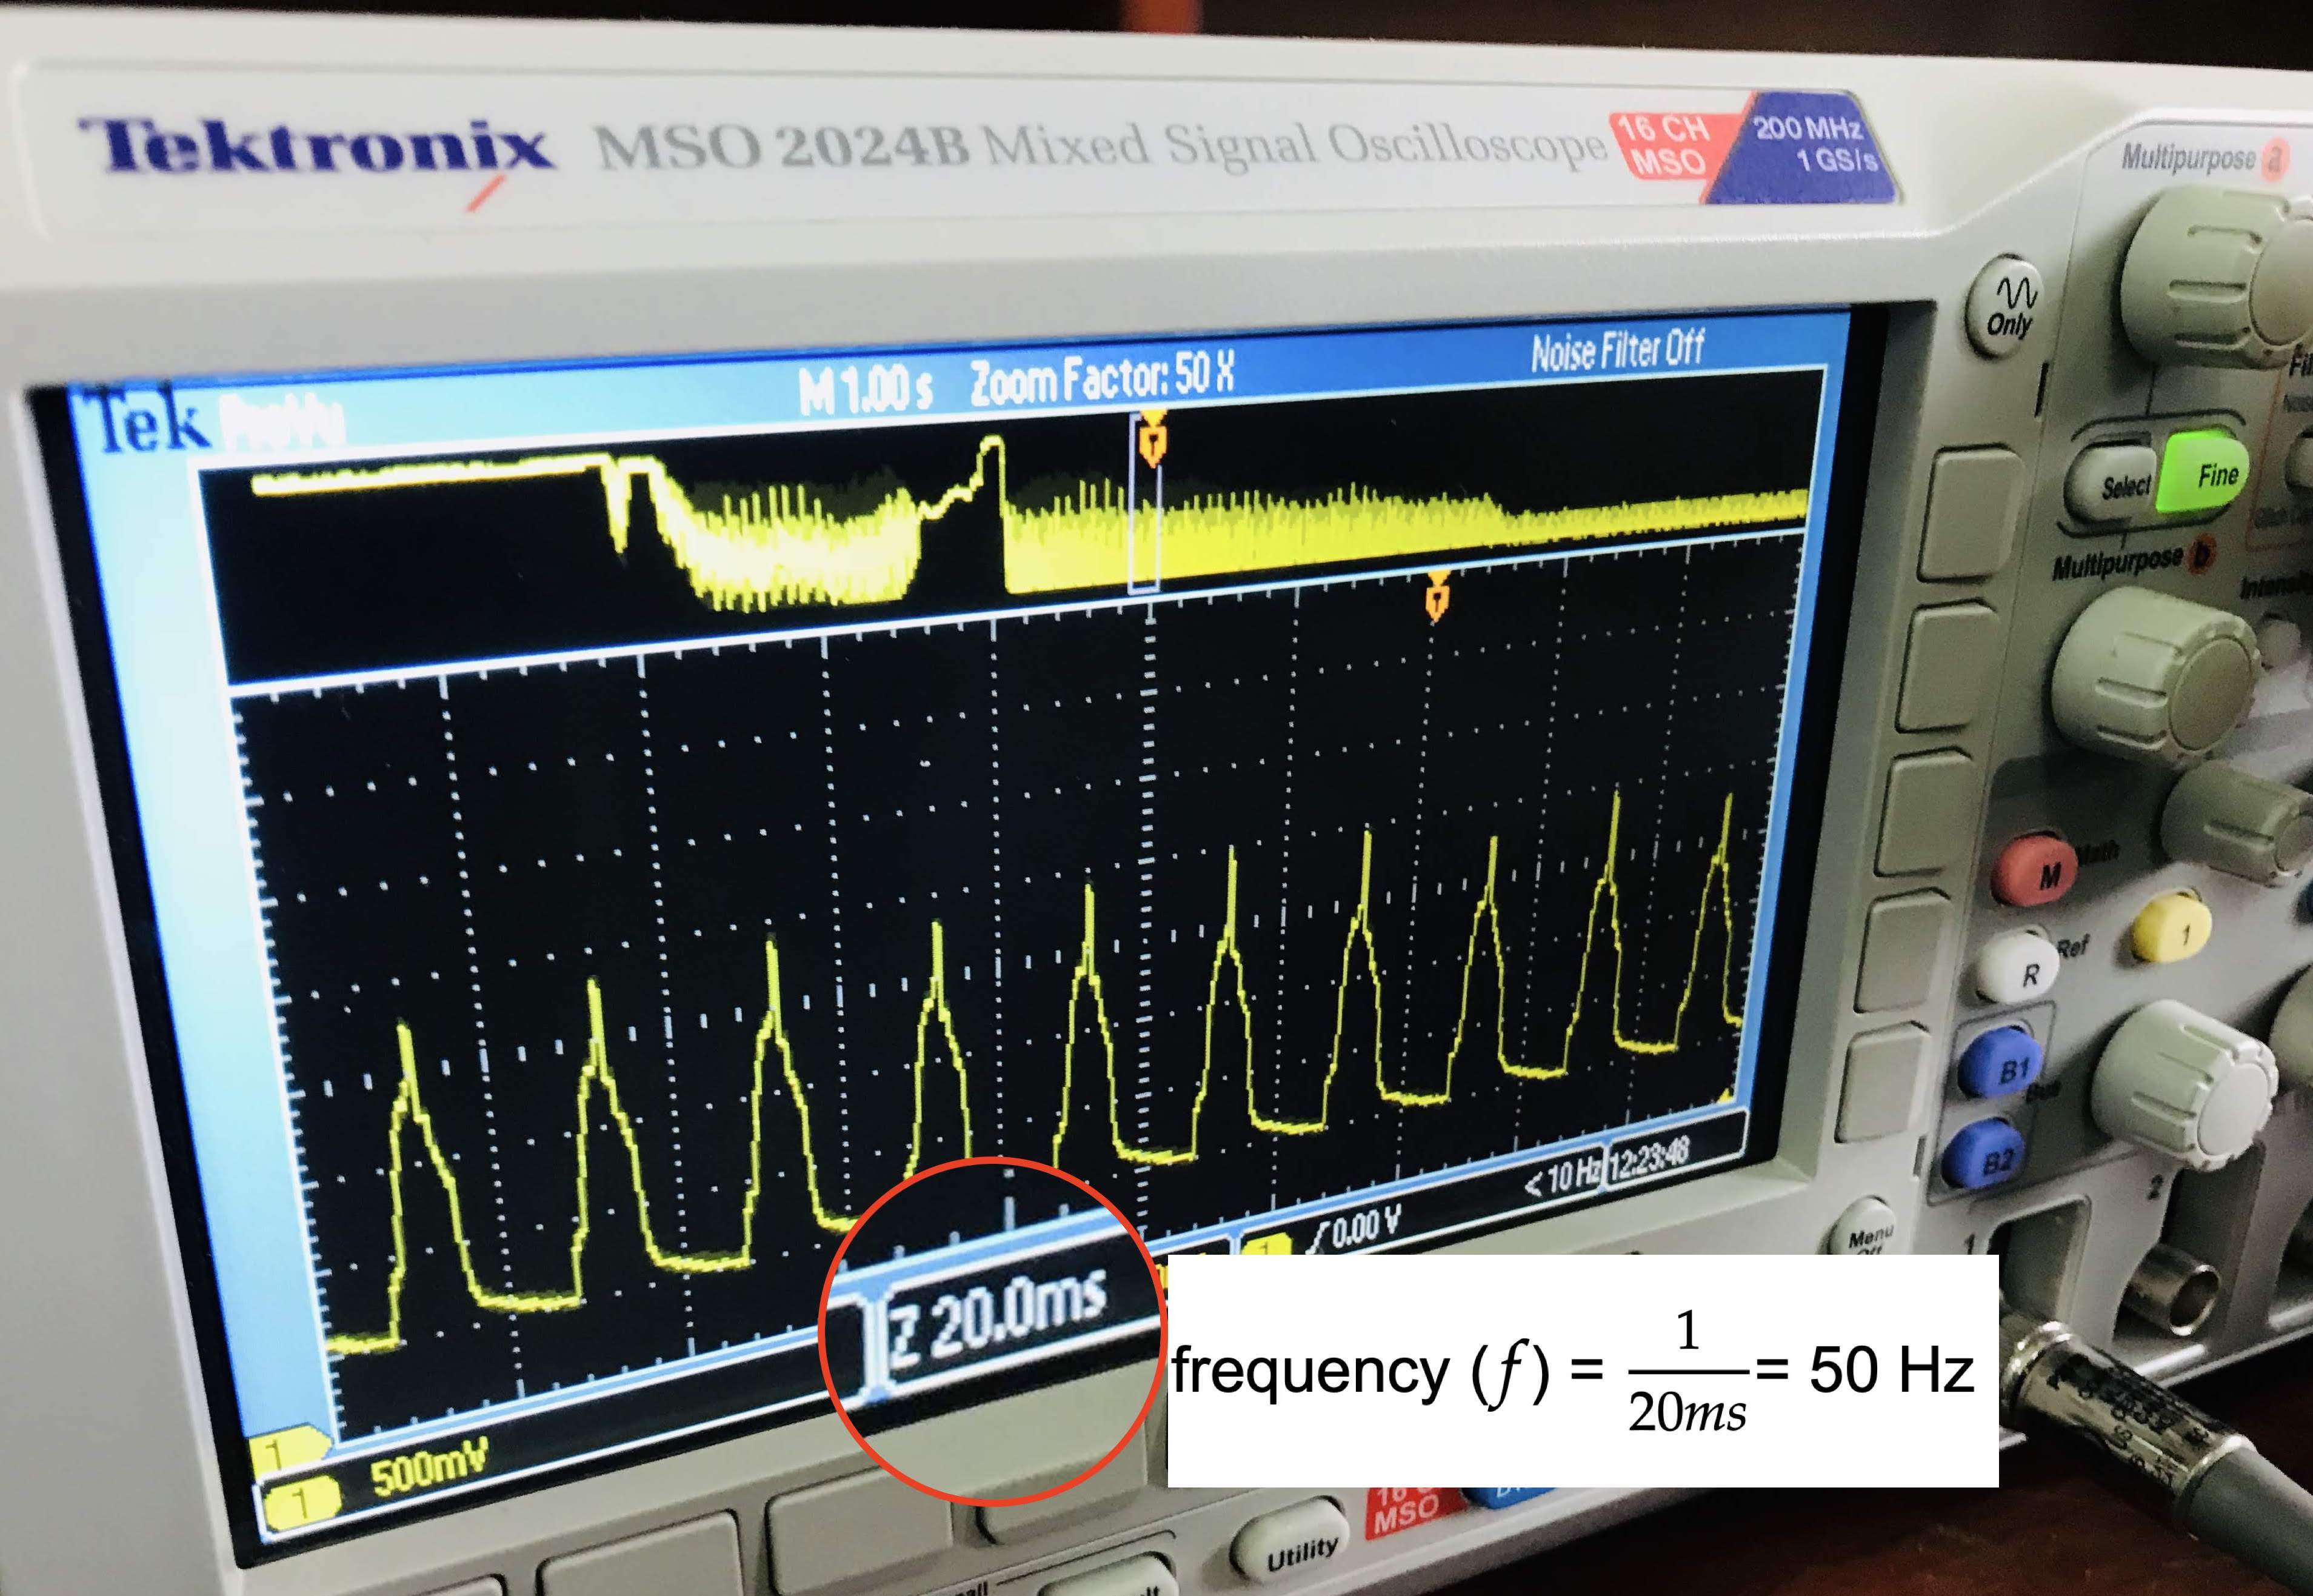
\includegraphics[scale=0.11]{50-dom.jpg}



\subsubsection{With the active bandpass filter}
The initial circuit was modified into an active bandpass filter circuit by calculating the necessary values as shown in \hyperref[sec:4.2.1]{4.2.1}.Next, using the signal generator, we observed the characteristics of our filter circuit from the digital oscilloscope. The responses were as follows; Observation: The amplitudes of the frequencies at the cut of frequencies were gradually reduced.\footnote{The required range of frequencies 50-140bpm (0.83 - 2.33Hz) were passed without much attenuation}

\begin{figure}[h]

	\begin{tabular}{ccc}

\subfloat[0.1Hz]{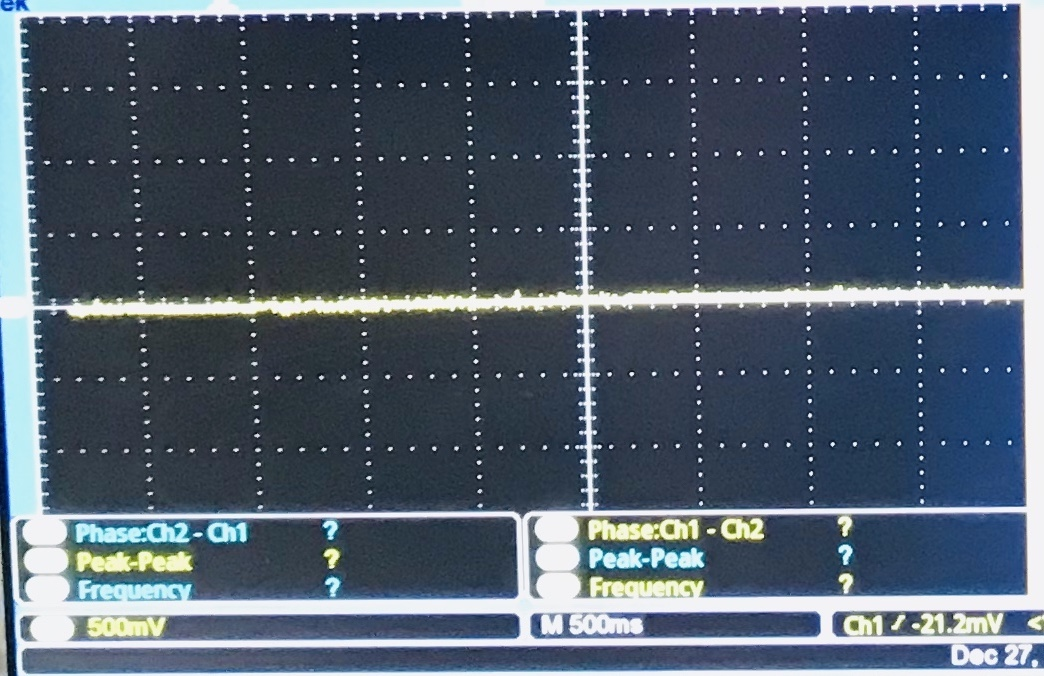
\includegraphics[width = 1.9in]{0-1.jpg}}&
\subfloat[0.2Hz]{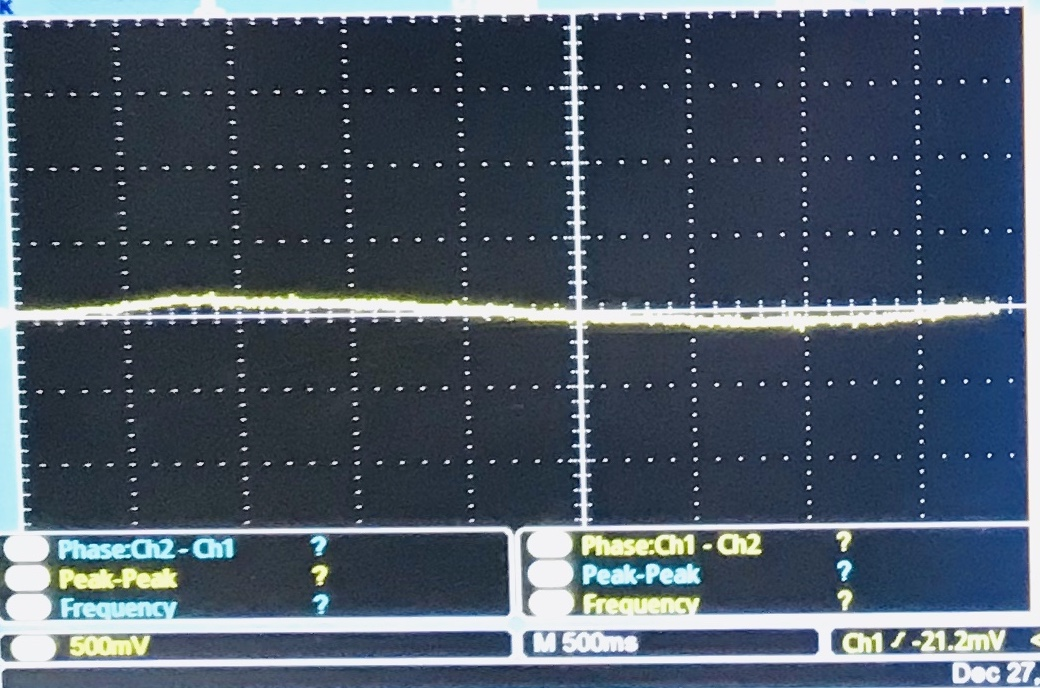
\includegraphics[width = 1.9in]{0-2.jpg}}&
\subfloat[0.3Hz]{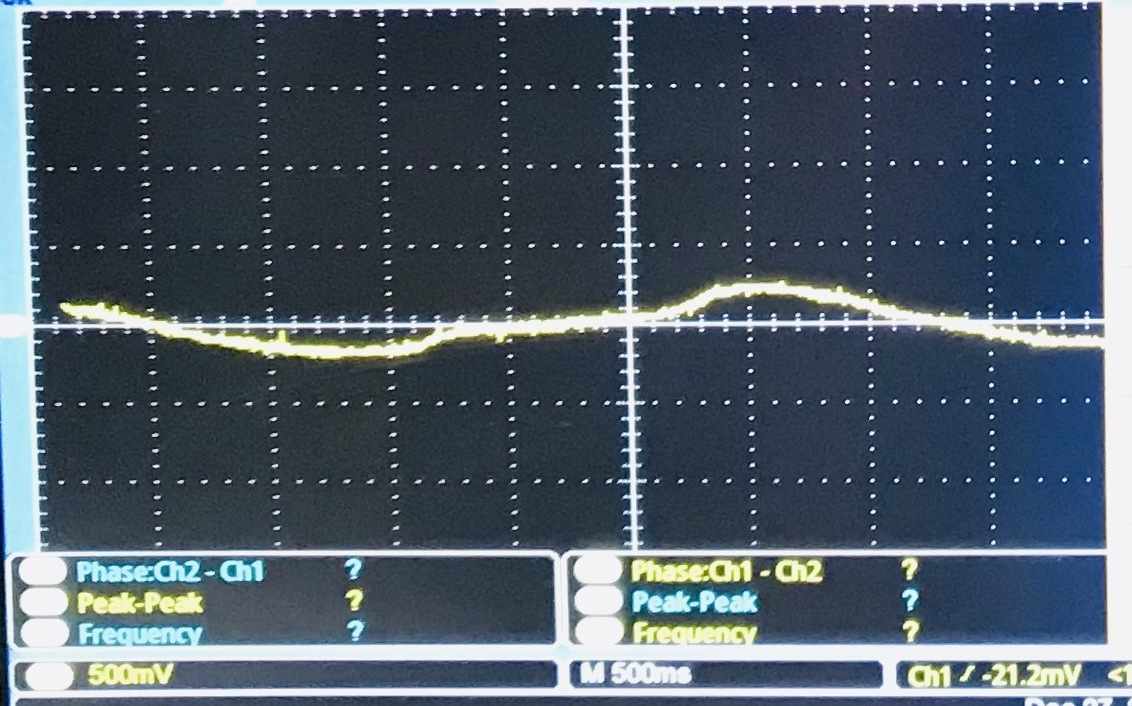
\includegraphics[width = 1.9in]{0-3.jpg}}\\

\end{tabular}
\end{figure}

\begin{figure}[h]
	\ContinuedFloat*
	\begin{tabular}{ccc}

\subfloat[0.4Hz]{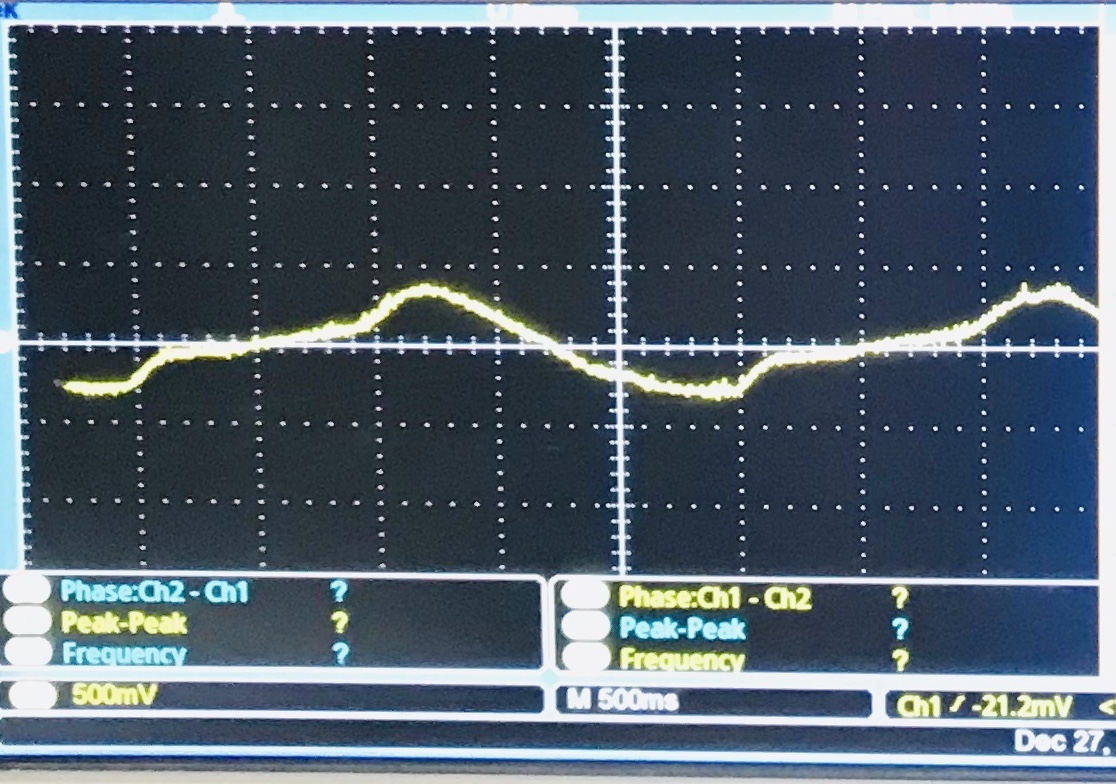
\includegraphics[width = 1.9in]{0-4.jpg}}&
\subfloat[0.5Hz]{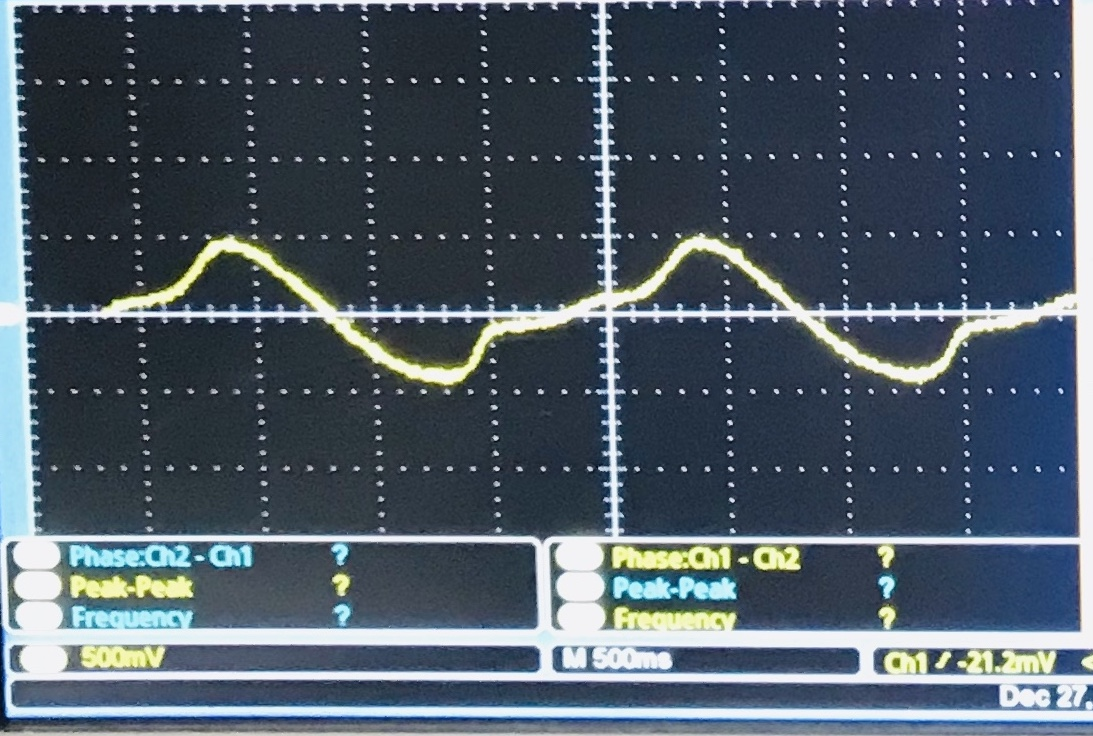
\includegraphics[width = 1.9in]{0-5.jpg}}&
\subfloat[0.6Hz]{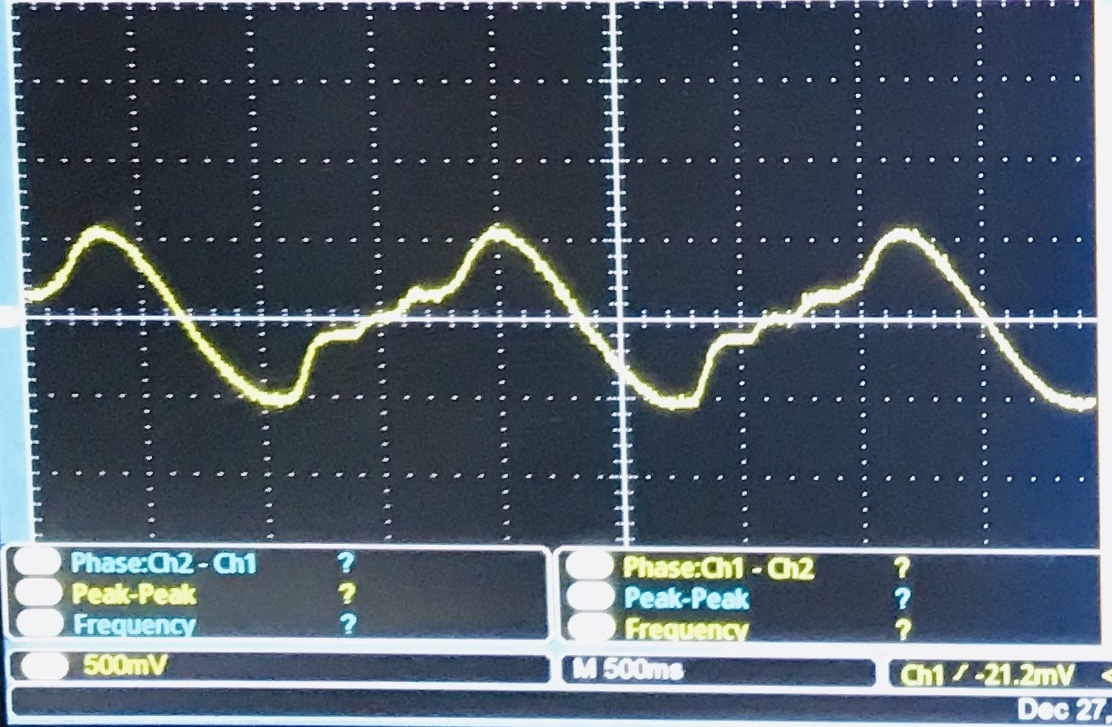
\includegraphics[width = 1.9in]{0-6.jpg}}\\

\subfloat[0.7Hz]{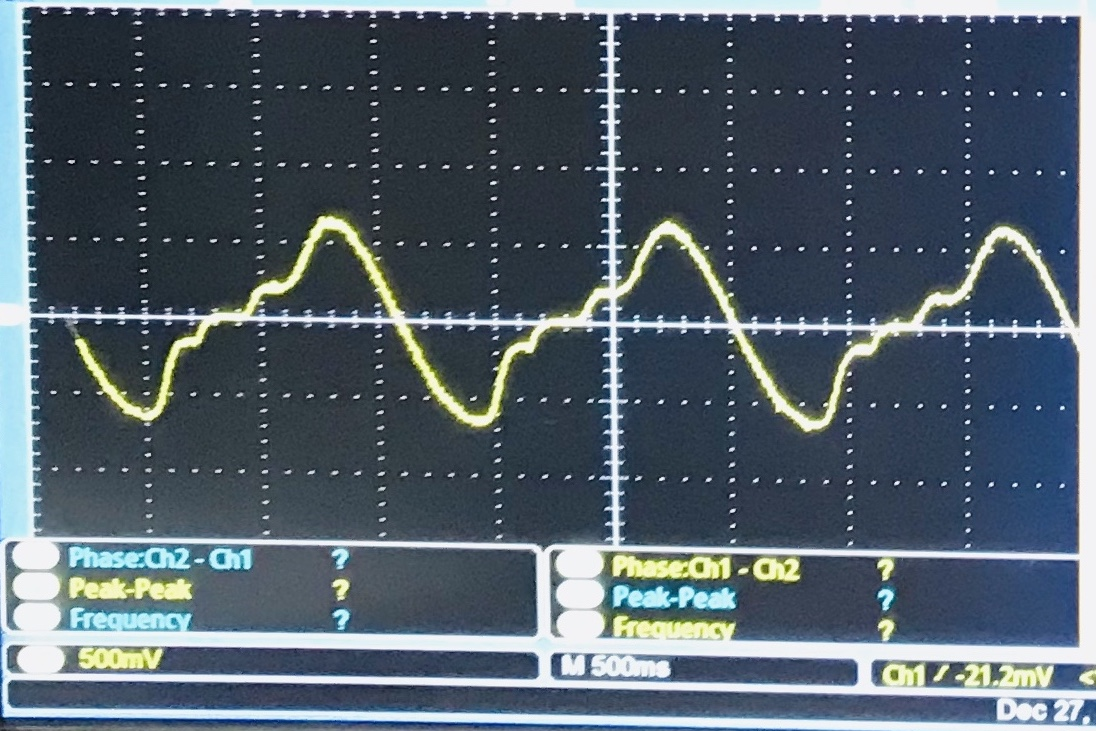
\includegraphics[width = 1.9in]{0-7.jpg}}&
\subfloat[0.9Hz]{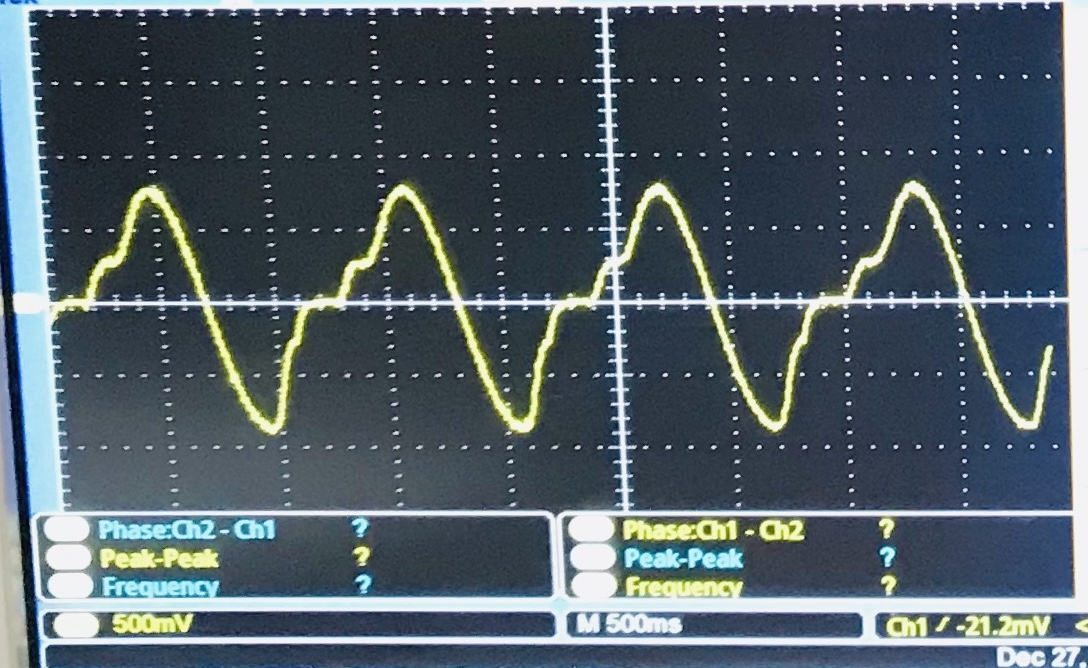
\includegraphics[width = 1.9in]{0-9.jpg}}&
\subfloat[1.2Hz ]{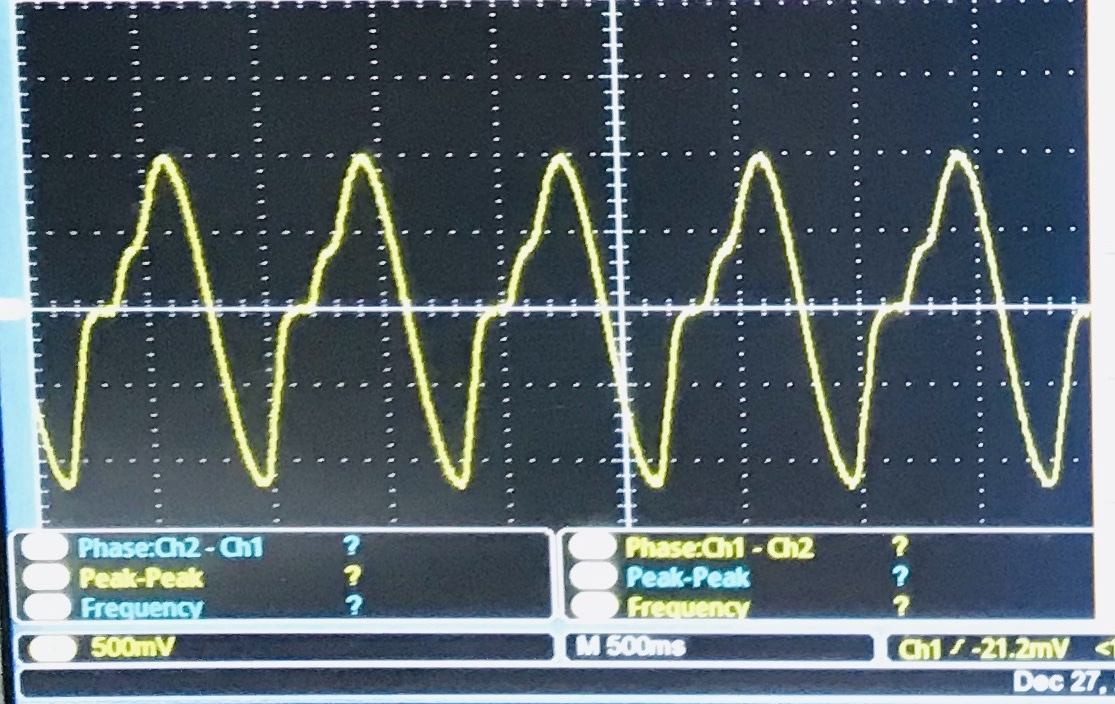
\includegraphics[width = 1.9in]{1-2.jpg}}\\

\subfloat[1.5Hz]{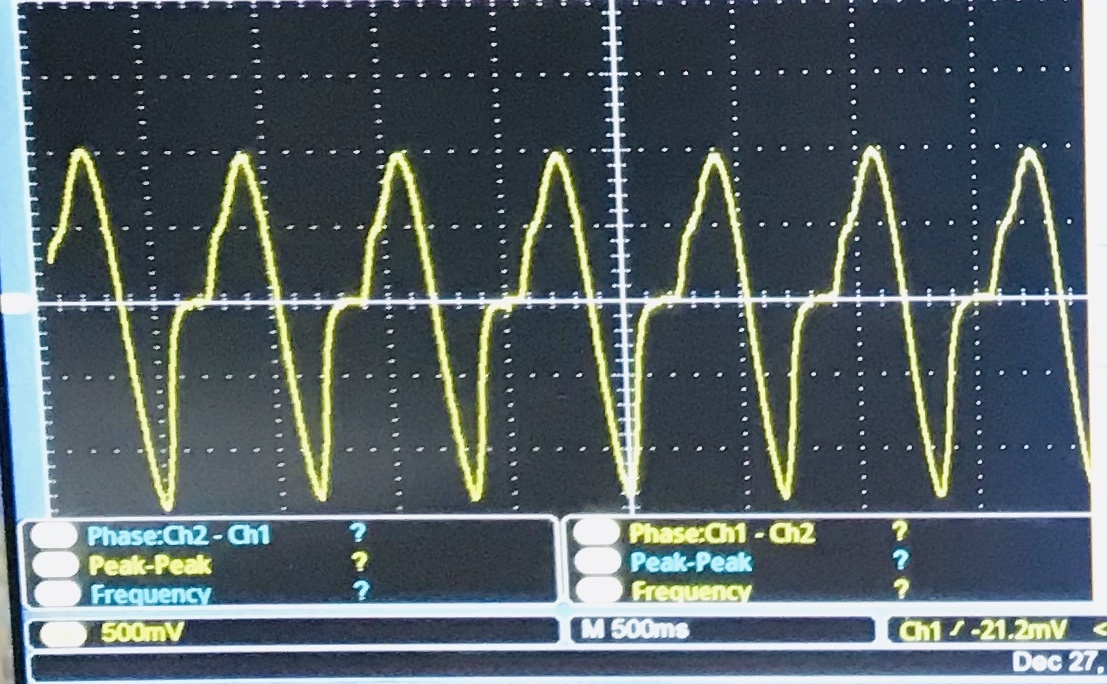
\includegraphics[width = 1.9in]{1-5.jpg}}&
\subfloat[2Hz]{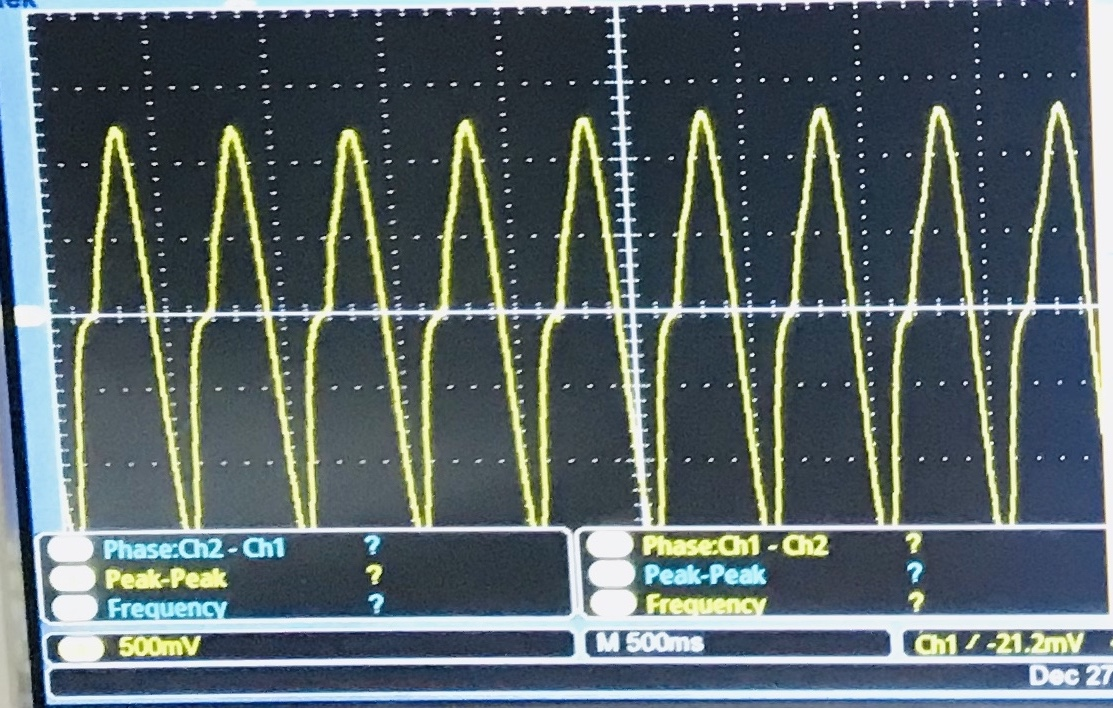
\includegraphics[width = 1.9in]{2.jpg}}&
\subfloat[2.5Hz]{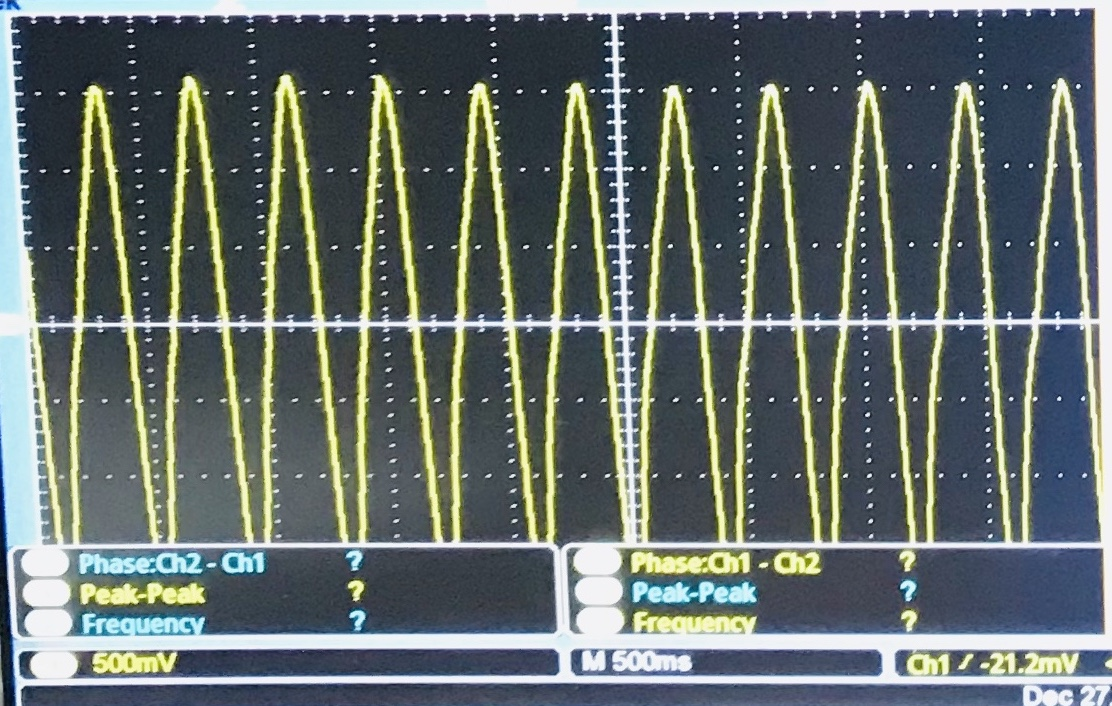
\includegraphics[width = 1.9in]{2-5.jpg}}\\

\subfloat[6Hz]{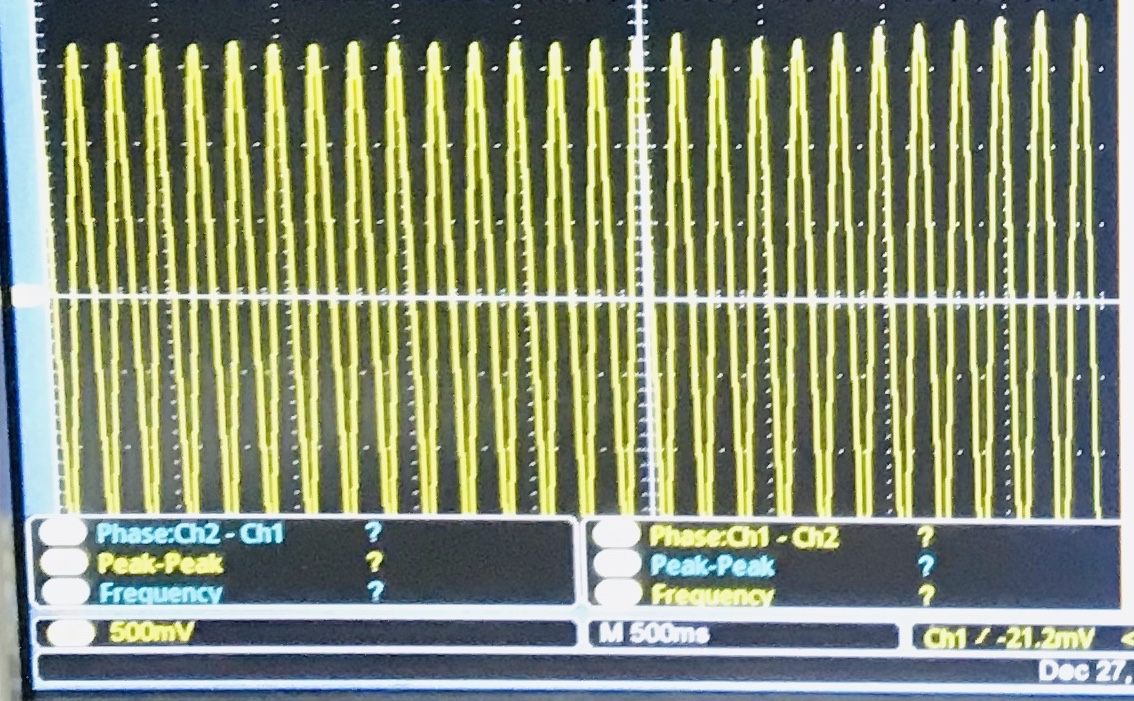
\includegraphics[width = 1.9in]{6.jpg}}&
\subfloat[10Hz]{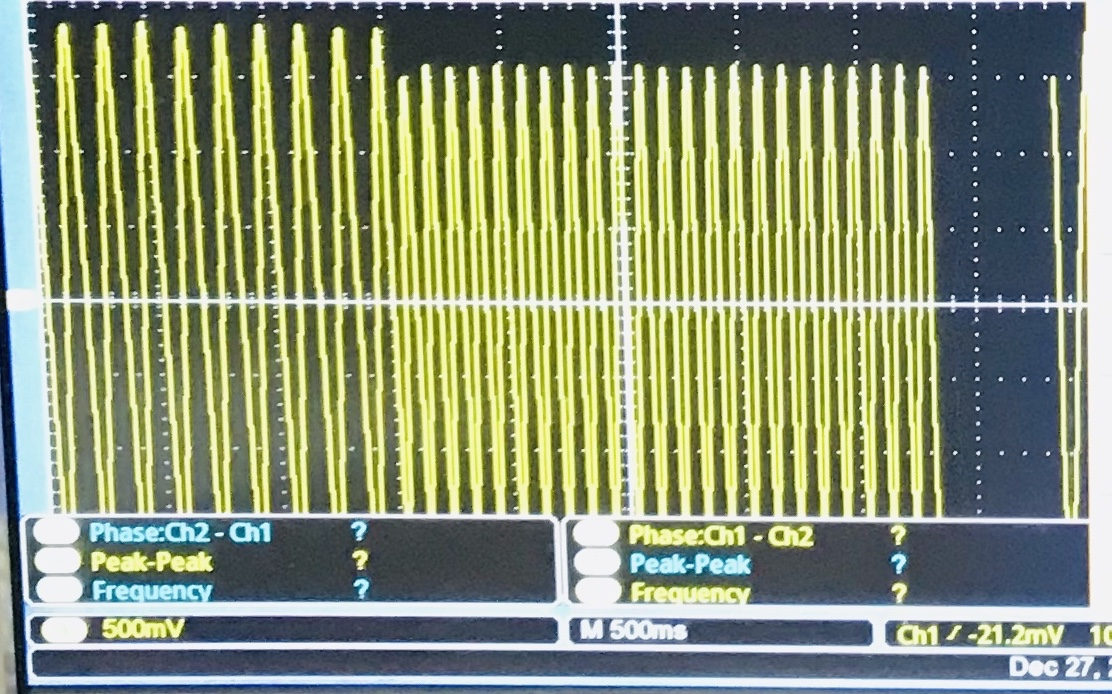
\includegraphics[width = 1.9in]{10.jpg}}&
\subfloat[15Hz]{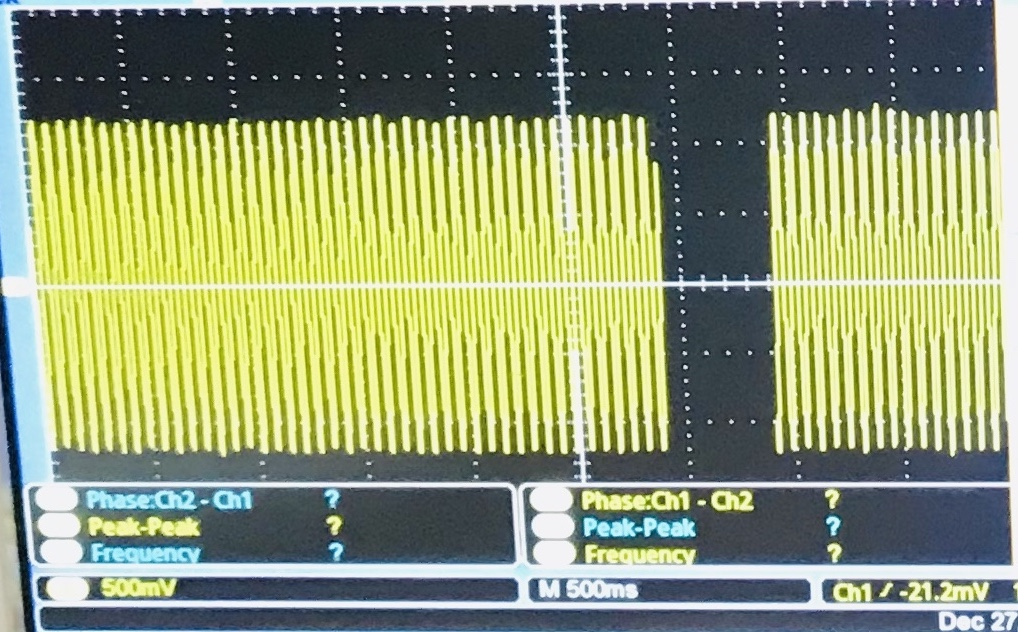
\includegraphics[width = 1.9in]{15.jpg}}\\

\end{tabular}
\caption{Frequency response of the bandpass filter}
	\end{figure}
\clearpage



By the observations above we were able to verify that the response of this circuit can be given by the graph below:

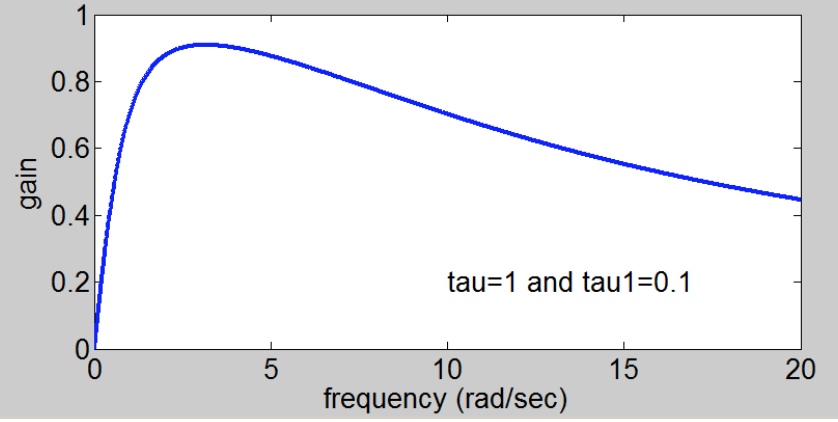
\includegraphics[scale=0.5]{bandpass.jpg}

\subsubsection{Obtaining a threshold value}

During testing, it was observed that due to ambient lighting conditions and movement of the patients’ finger placement between the LED and photodiode sudden amplitude changes can occur. 

It was evident that a hardcoded threshold value will not count the number of peaks accurately. Therefore, the calibration algorithm which was explained in \hyperref[sec:4.3.2]{4.3.2} determines a threshold value per user.


\begin{figure}[!htbp]
	
	\begin{tabular}{ccc}
\subfloat[Variying amplitudes]{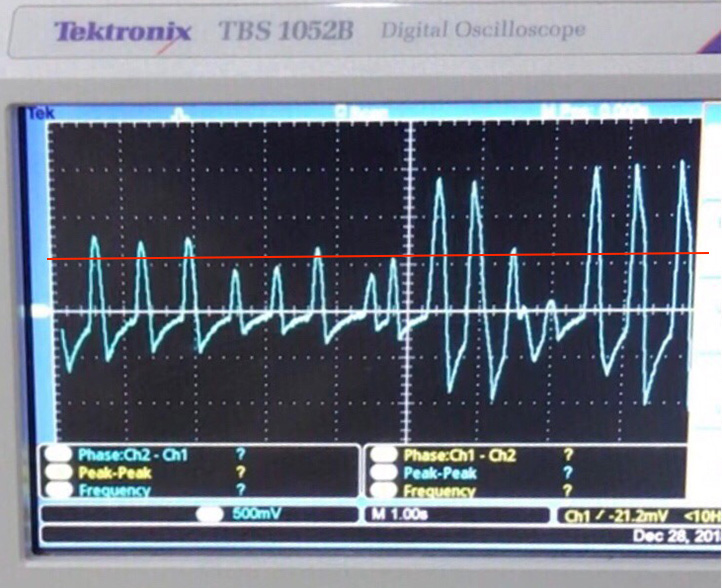
\includegraphics[width = 2.9in]{test1.jpg}}&
\subfloat[Amplitude Gradually decreasing]{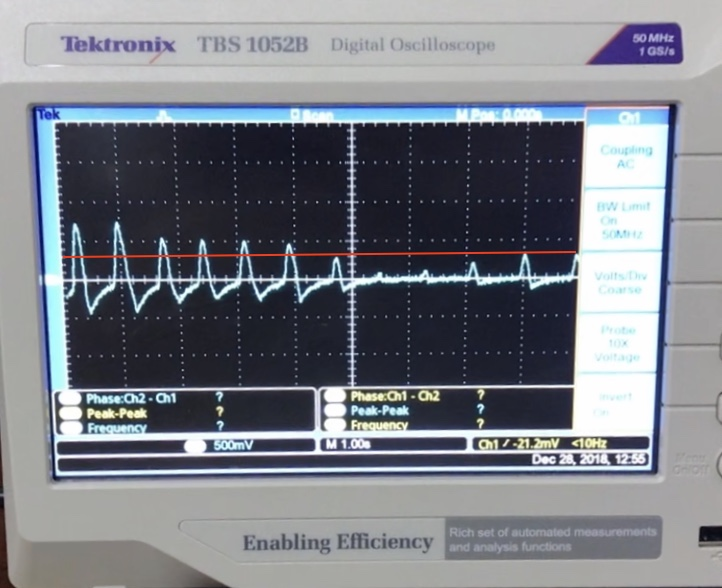
\includegraphics[width = 2.9in]{test2.jpg}}\\
	\end{tabular}
	\end{figure}
	
	

	\begin{wrapfigure}{L}{0.8\textwidth}
		\centering
		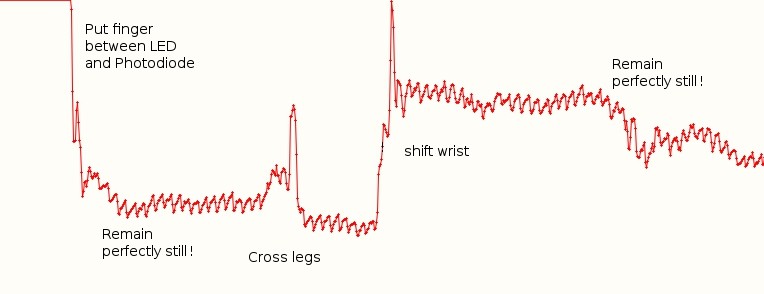
\includegraphics[width=0.75\textwidth]{breadboardmonitorwaveform.jpg}
		\caption{How PPG Varies\cite{analomy_pulse_sensor}}
		\end{wrapfigure}


		

\label{sec:results}
\begin{figure}[!htbp]
	\centering
	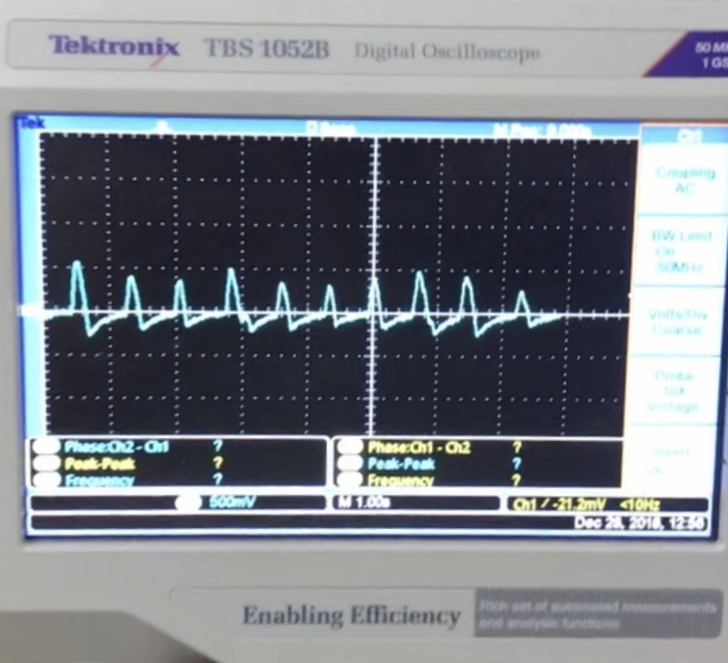
\includegraphics[scale = 0.35]{res1.jpg}
	\caption{Filtered Waveform}
\end{figure}

\clearpage

\begin{circuitikz}
	\draw
	(0,0) to[R, o-o] (2,0)
	(4,0) to[vR, o-o] (6,0)
	(0,2) to[transmission line, o-o] (2,2)
	(4,2) to[closing switch, o-o] (6,2)
	(0,4) to[european current source, o-o] (2,4)
	(4,4) to[european voltage source, o-o] (6,4)
	(0,6) to[empty diode, o-o] (2,6)
	(4,6) to[full led, o-o] (6,6)
	(0,8) to[generic, o-o] (2,8)
	(4,8) to[sinusoidal voltage source, o-o] (6,8)
	;
	\end{circuitikz}
\lipsum[1]


\newpage
\section{Discussion}
\lipsum[2]


\newpage
\section{Online Materials}
The project has been open sourced on Github. All the diagrams, schematics, PCB designs can be found through our repository.\\\\
\faGithub\href{https://github.com/ramithuh/Pulse-Sensor}{ https://github.com/ramithuh/Pulse-Sensor}.

 
\newpage
%	Bibliography


%----------------------------------------------------------------------------------------
\bibliography{biblist}{}
\bibliographystyle{plain}
\end{document}